\documentclass[10pt,a4paper]{article}
\usepackage[utf8]{inputenc}
\usepackage{url}
\usepackage[english]{babel}
\usepackage{amsmath}
\usepackage{amsfonts}
\usepackage{amssymb}
\usepackage{graphicx}
\usepackage[left=2cm,right=2cm,top=2cm,bottom=2cm]{geometry}
\author{Andres Chaves}
\title{Research Proposal}

\begin{document}
 \title{Research Proposal}
 \author{Andres Chaves (706801) \\
  \multicolumn{1}{p{.7\textwidth}}{\centering\emph{Melbourne School of Information\\The University of Melbourne}}}
 \maketitle

\begin{abstract}
    The purpose of this documents will be to stablish the context and bases of the research proposal which applies concepts of Machine Learning into Network Management Systems.
   \\\\
   Throughout this document one will read the relevance of the research, how will the concepts of Machine Learning will be applied to Event-processing Network Management Systems and finally what are the expected results.
\end{abstract}


\tableofcontents

  
 \section{Introduction}
 There is no doubt of the strong development and evolution of Information Technologies in modern world. Nowdays we have access to computing devices in whatever form (Supercomputer, Laptops, Tablets, Mobile, etc.) in conjunction with  advanced distributed information systems.
 \\\\
 But all this evolution could not be accomplished without a key component: Computer Networks. Networks make possible for data exchange and service consumption and side by side with Information Technology, networking evolved from simple small low bandwidth networks, to high speed wired and wireless ones connecting all the world.
 \\\\
 These huge networks require a set of practices, tools and knowledge in order to garantee the availability and speed required by the clients. A discipline called Network Management arised to address all these concerns and nowdays network management comprises all the practices and activities that a carrier must perform in order to fulfill its Service Level Agreements (SLAs) with its clients.
 \\\\
 From the information systems perspective, Network Management requires a set of systems called Network Management Systems (NMS) designed to administer either all or a part of the network. These administration comprises a set of functions: Fault Management, Performance Management, Configuration Management and Security Management among others.
 \\\\
 Fault Management involves how to detect, classify and inform the Network Operator about conditions that affect or may affect the network services, both from availability and performance perspective.
 \\\\
 One of the recent challenges in Network Management is how to monitor ever bigger networks, currently the network devices that a carrier must administer is measured in the range of thousands to millons. With this size a key desired function is only show the relevant alarms that matter to the network operators.
 \\\\
 One possible approach to analyse, classify and display only the relevant events to the operator is by the use of a machine learning system that can help the network operator in the processing of events and thus augmenting the network management capacity with the same engineering team.
 \\\\
 This project intends to advance in this approach and measure the benefits of the use of a machine learning system to fault management.

 \section{Objective}
The objective of this project is to analyse how machine learning technologies can be applied to Network Management Systems, specifically event/fault management systems in order to provide more quality and key events to the network operator and thus increase the network management capacity of a Network Operation Center.

The Machine Learning technique will be used for correlation rules generation as an id to the human expert. The objective is not to replace the judge and knowledge of the engineer but quickly help him in discovering what correlation rules may be applied to reduce the ratio alarm to operator.
 
  \section{Technical Approach}
A generic SNMP Network Management System is a stream based system that conceptually can be divided in several stages: Alarm reception, alarm translation and enrichment, event correlation and event presentation. A conceptual schema can be seen on Figure \ref{fig:nms_generaldiagram}
\\\
\begin{figure}[H]
 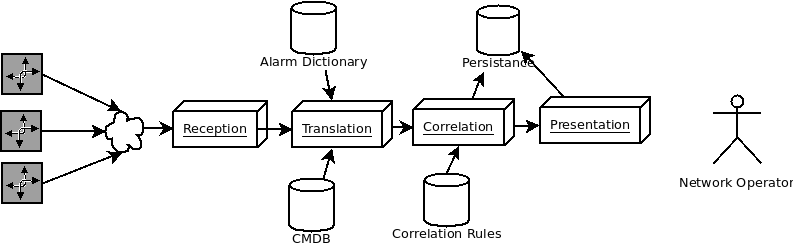
\includegraphics[scale=0.5]{NMS_GeneralDiagram.png}
  \centering
  \caption{\textit{A schematic of a generic Network Management System}}
  \label{fig:nms_generaldiagram}
\end{figure}	

For our testing environment we are going to use several open source components to simulate a Management System. These are:

\begin{itemize}
  \item Net-SNMP: Net-SNMP is an open source Linux and Unix package that implements the SNMP protocol.\cite{netsnmp}
  \item SNMPTT: SNMPTT or SNMP-Trap Translator is an open source component that takes the SNMP trap (alarm) received by Net-SNMP and by using an alarm dictionary translate it into a more useful string. SNMPTT can also enrich the alarm from a database by executing a shell script.\cite{snmptt}
  \item SEC: SEC or Simple Event Correlator is an open source component that allows correlation of events streaming to the system.\cite{sec}
  \item MYSQL: MySQL is an open source relational database. For the purposes of this proposal, it will be used as storage for the Configuration Management Database.
\end{itemize}

The key work will be to apply Machine Learning techniques to the input stream arriving to SEC in order to infer what will be the proper rules to configure this correlation.

There will be also a recording of live networking event data to be used as a sample. For the purposes of the research the recording will be only for alarms of Layer 3 Routing Devices, but the concepts applied must apply to any kind of device/network.
\\\\
The recording will have a flag to indicate whether the operator consider the alarm is important or not. This field along with the context of the alarm (device, port, location, label) will be the input to the different machine learning algorithms. The output of the algorithms will be a set of infered rules, that will be again evaluated and tested.

The proposed components can be seen on figure \ref{fig:ml_componentdiagram}

\begin{figure}[H]
 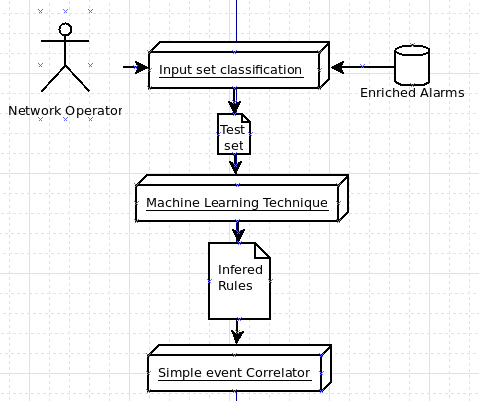
\includegraphics[scale=0.5]{ML_ProposedComponents.png}
  \centering
  \caption{\textit{Proposed Machine Learning Application}}
  \label{fig:ml_componentdiagram}
\end{figure}	

  \section{Time Table and Deliverables}
  \section{Literature Review}

\begin{thebibliography}{9}

\bibitem{netsnmp}Net-SNMP website, \url{http://www.net-snmp.org/}.
\bibitem{snmptt}SNMPTT website, \url{http://snmptt.sourceforge.net/docs/snmptt.shtml}.
\bibitem{sec}SEC website, \url{http://simple-evcorr.sourceforge.net}.
\bibitem{lamport94}
  Leslie Lamport,
  \emph{\LaTeX: a document preparation system}.
  Addison Wesley, Massachusetts,
  2nd edition,
  1994.

\end{thebibliography}
    
\end{document}